% !TEX program = xelatex
\documentclass{article}
\usepackage[utf8]{inputenc}
\usepackage{amsmath}
\usepackage{relsize}
\usepackage{amssymb}
\usepackage{mathabx}
\usepackage{amsthm}
\usepackage{graphicx}
\usepackage[usenames,dvipsnames]{xcolor}
\usepackage{subcaption}
\newcommand{\kacper}[1]{ \bf  { \color{Orchid}{Kc: #1}}  }

\newtheorem{definition}{Definition}
\newtheorem{lemma}{Lemma}
\newtheorem{Theorem}{Theorem}
\newtheorem{example}{Example}
\newtheorem{statement}{Statement}
\newtheorem{corollary}{Corollary}
\newtheorem{test}{Test}
\newtheorem{proposition}{Proposition}

\newtheorem*{remark}{Remark}
\newenvironment{claim}[1]{\par\noindent\underline{Claim:}\space#1}{}
\newenvironment{claimproof}[1]{\par\noindent\underline{Proof:}\space#1}{\hfill $\blacksquare$}
\newcommand{\ev}{\mathbb{E}}
\title{Testing MCMC convergence}
\author{}
\date{}

% TODO 
% Wrong disitbution under null if ratio is not good


\begin{document}

\maketitle

The purpose of a goodness of fit test is to show whether a distribution
$p$ matches some reference distribution $q$, which is in our case
assumed to have a density wrt the Lebesgue measure, $dq(x)=q(x)dx$
(in fact, as we will see, it makes most sense for it to be in the
exponential family).

\section{Kernel One Sample Test}
In the following section we derive kernel one sample test. The test is applicable to family of distributions $\mathcal{P}$, on $d$-dimensional plane, where $p \in \mathcal{P}$ satisfy two conditions: \\ 
(i) $\ev \log p(Z)    <\infty$ for any random variable $Z$; \\
(ii) $\ev   \| \nabla \log p(X) \|^2_2  $  for $X \sim p$,\\
where $\nabla f(x) = \left( \frac{\partial f(x)} {\partial x_1}l, \cdots, \frac{\partial f(x)} {\partial x_d} \right)$ and $\| \cdot \|_2$ is norm $l_2$ norm of $R^d$ space. Let $k$ be a bounded, symmetric, cc-universal \cite{sriperumbudur2011universality}  kernel  and $\mathcal{F}$  the Reproducing Kernel Hilbert Space  associated with it. In addition, we assume that for any random variable $Z$ \\ 
(iii) $\ev \left(\frac{\partial^{2} k(Z,Z) }{dx_i dx_{i+d} }\right)^2<\infty$. Let $\mathcal{F}^d$ be a product space, with standard inner product i.e. for $f,g \in \mathcal{F}^d$,  $\langle f,g \rangle = \sum_{i=1}^d \langle f_i,g_i \rangle$.


\paragraph{Stein operator.}
We proceed as similarly to \cite{mackey2015multivariate,stein1972} and use Stein operator to characterize discrepancy between measures.


Similarly to \cite{mackey2015multivariate} we study the operator $T_p$ acting on $R^d$ valued functions, 
\[
T_{p} f=  \sum_{i=1}^{d} \left( \frac{\partial \log p(x)}{ \partial x_i} f_i(x)+\frac{\partial f_i(x)}{ \partial x_i} \right).
\]
In contrast to \cite{mackey2015multivariate} we restrict ourselves  to $f \in \mathcal{F}^d$. Following \cite{mackey2015multivariate} we first show  that for all $f \in F^d, \ev (T_{q}f)(X) = 0$ (Lemma \ref{lem:easy}), and next, for any random $Z$ variable, we define Stein discrepancy between $X \sim p$ and $Z$ 
\[
 S(Z,\mathcal{F},p) = \sup_{f \in F^d,\| f \|<1} \ev (T_{p}f) (Z)  = \sup_{ f \in F^d } \ev (T_{p}f)(Z) - \ev (T_{p}f) (X).
\]
In Theorem \ref{th2} we show that  $S(Z,\mathcal{F},p)$ captures difference between probability measures. Contrary to to \cite{mackey2015multivariate}, we don't need to approximate $S(Y,\mathcal{F},p)$ (step 2 and 3 in section 3), since we can calculate it explicitly \ref{th1}. 



\begin{definition}
For any $x \in R^d$, define a vector valued function function  $\xi: R^d \to R^d$,
\[
 \xi(x,t) =\left[ \nabla \log p(x) k(x,t)+\nabla_1 k(x,t)\right]
\] 
where $\nabla \log p(x) = \left( \frac{\partial \log p(x)}{ \partial x_1}, \cdots , \frac{\partial \log p(x)}{ \partial x_d} \right)$ and 
$  \nabla_1 k(x,t) = \left( \frac{\partial k(x,t)}{ \partial x_1}, \cdots , \frac{\partial  k(x,t)}{ \partial x_d} \right)$. 
\end{definition}

\begin{statement}
\label{lem:WellDefined}
 $\xi(x,\cdot)$ is an element of the reproducing kernel Hilbert space $\mathcal{F}^d$.
\end{statement}
\begin{proof}
 We use the proof on p. 132 of \cite[Corollary 4.36]{SteChr08} to see that for all $x \in R^d$ each entry of $\nabla_1 k(x,\cdot)$ is in $\mathcal{F}$. $\frac{\partial \log p(x)}{ \partial x_i} k(x,t) \in \mathcal{F}$, since $k(x,t) \in\mathcal{F}$ and $\frac{\partial \log p(x)}{ \partial x_i}$ is a scalar. 
\end{proof}


\begin{statement}
\label{lem:BochnerInt}
$\xi(x,\cdot)$ is Bochner integrable with respect to any probability measure.
\end{statement}

\begin{proof}
It is sufficient to check that coefficients of $\xi$ are Bochner integrable  (\cite[Definition A.5.20]{SteChr08}). first we check that for random any variable $Z$
\[
\ev \left\Vert \frac{\partial \log p(Z) }{\partial x_i} k(Z,\cdot)\right\Vert^2 = \| k \|_{\infty}\ev \left( \frac{\partial \log p(Z) }{\partial x_i} k(Z,Z) \right)^2 <\ev   \| \nabla \log p(X) \|^2 <\infty,
\]
which follows form assumption (i) and boundedness of the kernel. Next we check that 
\[
\ev \left\Vert \frac{\partial k(Z,\cdot)}{\partial x}\right\Vert^2 =\ev \left(\frac{\partial^{2} k(Z,Z) }{dx_i dx_{i+d} }\right)^2<\infty,
\]
which follows from assumption (iii). 
\end{proof}

\begin{corollary}
 For any random variable $Z$, expected value of $\xi(Z)$ is is element of $\mathcal{F}^d$.
\end{corollary}


\begin{lemma}
\label{lem:inner}
For any random variable $Z$, expected value of Stein operator coincides with inner product of $f$ and expected value of $\xi(Z)$ i.e. 
\begin{align}
\ev T_{p} f(Z) = \langle f ,\ev \xi(Z) \rangle_{\mathcal{F}^d}  =\sum_{i=1}^d \langle f_i, \ev \xi_i(Z) \rangle_{\mathcal{F}}
\end{align}
\end{lemma}

\begin{proof}
  \begin{align*}
 \left\langle f_i, \ev \xi_i(Z) \right\rangle  &= \left\langle f_i,\ev \left[ \frac{\partial \log p(Z)}{ \partial x_i} k(Z,\cdot)+ \frac{\partial k(Z,\cdot)}{ \partial x_i}\right]\right\rangle_{\mathcal{F}} \\
  &= \ev \left\langle f_i, \frac{\partial \log p(Z)}{ \partial x_i} k(Z,\cdot)+ \frac{\partial k(Z,\cdot)}{ \partial x_i}\right\rangle_{\mathcal{F}} \\
 &=\ev \left[ \frac{\partial \log p(Z)}{ \partial x_i} f_i(Z)+ \frac{\partial f(Z)}{ \partial x_i}\right]\\
\end{align*}
The second equality follows form the fact that linear operator $\langle f_i , \cdot \rangle_{\mathcal{F}}$ can be interchanged with Bochner integral and the fact that $\xi$ is Bochner integrable (Lemma \ref{lem:BochnerInt}). The last equality is application of reproducing property.    
\end{proof}

\begin{lemma}
$S(X,\mathcal{F},p)^2 = \langle \ev \xi(X), \ev \xi(X) \rangle_{\mathcal{F}^d } $. 
\end{lemma}
\begin{proof}
 Using the Lemma \ref{lem:inner} we see that 
 \begin{align}
  S(X,\mathcal{F},p) = \sup_{f \in \mathcal{F}^d, \| f \| <1 } \langle f ,\ev \xi(X) \rangle_{\mathcal{F}^d},
 \end{align}
which was is attained at $f^* = \frac{\ev \xi(X)} {\| \ev \xi(X) \| } $. Notice that 
 \[
  \langle f^*, \ev \xi(X) \rangle  = \| \ev \xi(X) \|,
 \]
 which in turn implies that $S(X,\mathcal{F},p)^2 = \langle \ev \xi(X), \ev \xi(X) \rangle_{\mathcal{F}^d }$. 
%  
 \end{proof}



\begin{lemma}
\label{th1}
$S(X,\mathcal{F},p)^2$ can be written in a closed form. 
\end{lemma}

\begin{proof}
We use notation 
\begin{align*}
 \nabla_1 k(x,y) = \left( \frac{\partial k(x,y) }{\partial x_1}, \cdots, \frac{\partial k(x,y) }{\partial x_d} \right) \\
 \nabla_2 k(x,y) = \left( \frac{\partial k(x,y) }{\partial y_1}, \cdots, \frac{\partial k(x,y) }{\partial y_d} \right). \\ 
\end{align*}
and $\langle \cdot, \cdot\rangle_2 $ for inner product in $R^d$.
\begin{align*}
S(X,\mathcal{F},p)^2 & = \langle \ev \xi(X), \ev \xi(X) \rangle_{\mathcal{F}^d } \\
& = \langle \ev \left[\nabla \log p(X) k(X,\cdot)+\nabla_1 k(X,\cdot)\right] ,\ev \left[\nabla \log p(X) k(X,\cdot)+\nabla_1 k(X,\cdot)\right] \rangle_{\mathcal{F}^d } \\
& \overset{(b)}{=} \ev \langle   \nabla \log p(X_1) k(X_1,\cdot) + \nabla_1 k(X_1,\cdot) , \nabla \log p(X_2) k(\cdot,X_2) + \nabla_2 k(\cdot,X_2) \rangle_{\mathcal{F}^d } \\
& = \ev\langle \nabla \log p(X_1) , \nabla\log p(X_2) \rangle_{2} k(X_1,X_2) + \ev \langle \nabla p(X_2),  \nabla_1 k(X_1,X_2) \rangle_{2} \\
  & \quad +  \ev \langle \nabla  \log p(X_1), \nabla_{2}  k(X_1,X_2) \rangle_{2} +  \ev\ \langle  \nabla_1 k(X_1,X_2), \nabla_2 k(X_1,X_2) \rangle_{2}
\end{align*}
For (b) we have used the fact that the kernel is symmetric.
\end{proof}

\begin{Theorem}
\label{th2}
Suppose  $q,p \in \mathcal{P}$ and $Y \sim q$, $S(Y,\mathcal{F},p) = 0$ if and only if $p=q$.
\end{Theorem}

\begin{proof}
If $p=q$ then, by Lemma \ref{lem:easy}, $S(Y,\mathcal{F},p) = 0$. Suppose $p \neq q$. For each dimension of $\ev \xi(Y)$ We add and subtract $\log q(Y)$.  
\begin{align*}
 &\ev \left( \frac{\partial } {\partial x_i} \log p(Y) k(Y,\cdot) + \frac{\partial } {\partial x_i} k(Y,\cdot)  \right) \\
 &=\ev \left( \frac{\partial } {\partial x_i} ( \log  p(Y) + \log  q(Y)- \log  q(Y)  )  k(Y,\cdot)   + \frac{\partial } {\partial x_i} k(Y,\cdot) \right) = \\
 &= \ev \left(  \frac{\partial } {\partial x_i} (\log p(Y) - \log q(Y))k(Y,\cdot) \right) 
\end{align*}
We have used Lemma \ref{lem:easy} to see that 
\[
\ev \left( \frac{\partial } {\partial x_i} (  \log  q(Y)  )  k(Y,\cdot)   + \frac{\partial } {\partial x_i} k(Y,\cdot) \right) =0.
\]
We recognize that expected value of random  $ \frac{\partial } {\partial x_i} (\log p(Y) - \log q(Y))  k(Y,\cdot)$ is mean embedding  of a function $g(y) =  \frac{\partial } {\partial x_i} (\log \frac{p(y)}{q(y)})$  with respect to  the measure $q$. Since kernel $k$ is cc-universal this embedding is zero if and only if $g = 0$ which implies that 
\[
 \nabla \log \frac{p(y)}{q(y)} = (0,\cdots ,0)
\]
A constant vector filed of derivatives  can only be generated by a constant functions, so $\log \frac{p(y)}{q(y)} =C$, for some $C$, which implies that  $p(y) = e^C q(y)$. Since $p$ and $q$ integrates to one $C=0$ and so $p=q$.
\end{proof}



\section{Test}

\paragraph{$V$-statistics.} The closed form formula for $S(X,\mathcal{F},p)^2$ (\ref{th1}) suggests that its approximation can be expressed as $V$-statistic. Given the observations $X=\left\{X_t\right\}_{t=1}^n$, a $V$-statistic of a symmetric function $h$ is given by 
\begin{equation}
\label{def:Vstat}
V_n = \frac{1}{n} \sum_{i,j=1}^n \nolimits h(X_i,X_j),
\end{equation}


The function $h$ is called a kernel of the $V$-statistic. It should cause no confusion with  

While such functions are usually called kernels in the literature, in this paper we reserve the term kernel for positive-definite functions taking two arguments. A core $h$ is said to be $j$-degenerate if for each $z_1,\ldots,z_j$ $\ev h(z_1,\ldots , z_j , Z_{j+1}^*,\ldots ,Z_m^*) = 0,$ where $Z_{j+1}^*,\ldots,Z_m^*$ are independent copies of $Z_1$. If $h$ is $j$-degenerate for all $j\leq m-1$, we will say that it is \emph{canonical}. For a one-degenerate core $h$, we define an auxiliary function $h_2$, called the second component of the core, and given by $h_2(z_1,z_2) = \ev h(z_1,z_2, Z_3^*,\ldots, Z_m^*).$ Finally we say that $nV(h)$ is a normalized $V$-statistic, and that a $V$-statistic with a one-degenerate core is a degenerate $V$-statistic.  This degeneracy is common to many kernel statistics when the null hypothesis holds \cite{gretton2012kernel,gretton_kernel_2008,sejdinovic2013kernel}.

Our main results will rely on the fact that $h_2$ governs the asymptotic behaviour of normalized degenerate $V$-statistics. Unfortunately, the limiting distribution of such $V$-statistics is quite complicated - it is an infinite sum of \emph{dependent} $\chi^2$-distributed random variables, with a dependence  determined by the temporal dependence structure within the process $\{Z_t\}$ and by the eigenfunctions of a certain integral operator associated with $h_2$ \cite{i._s._borisov_orthogonal_2009,chwialkowski2014kernel}. Therefore, we propose a bootstrapped version of the $V$-statistics which will allow a consistent approximation of this difficult limiting distribution.  

%\vspace{-4mm}
\paragraph{Bootstrapped $V$-statistic.} 
We will study two versions of the bootstrapped $V$-statistics  
\begin{align}
 V_{b1}(h,Z) = \frac{1}{n^m} \sum_{i \in N^m} \nolimits W_{i_1,n} W_{i_2,n} h(Z_{i_1},...,Z_{i_m}), \label{Vb1}\\ 
 V_{b2}(h,Z) = \frac{1}{n^m} \sum_{i \in N^m}  \nolimits \tilde W_{i_1,n}  \tilde W_{i_2,n} h(Z_{i_1},...,Z_{i_m}),\label{Vb2}
\end{align}
where $\{W_{t,n}\}_{1 \leq t \leq n }$ is an auxiliary wild bootstrap process and $\tilde W_{t,n} = W_{t,n} - \frac 1 n \sum_{j=1}^n W_{j,n}$. This auxiliary process, proposed by \cite{Shao2010,leucht_dependent_2013}, satisfies the following assumption:

\emph{Bootstrap assumption:} $\{W_{t,n}\}_{1 \leq t \leq n }$ is a row-wise strictly stationary triangular array independent of all $Z_t$ such that $\ev W_{t,n}=0$ and $\sup_{n} \ev|W_{t,n}^{2+\sigma}| < \infty$ for some $\sigma > 0$. The autocovariance of the process is given by $\ev W_{s,n} W_{t,n}=\rho(|s-t|/l_n)$ for some function $\rho$, such that $\lim_{u \to 0} \rho(u) = 1$ and $\sum_{r=1}^{n-1} \rho(|r|/l_n)= O(l_n)$. The sequence $\left\{l_n\right\}$ is taken such that $l_n=o(n)$ but $\lim_{n \to \infty} l_n = \infty$. The variables $W_{t,n}$  are $\tau$-weakly dependent with coefficients $\tau(r) \leq C \zeta^{\frac{r} {l_n}}$ for $r=1,...,n$, $\zeta \in (0,1)$ and $C\in\mathbb R$.

As noted in in \cite[Remark 2]{leucht_dependent_2013}, a simple realization of a process that satisfies this assumption is $W_{t,n} = e^{-1/l_n}W_{t-1,n} + \sqrt{1 -e^{-2/l_n}} \epsilon_t$
where $W_{0,n}$ and $\epsilon_1,\ldots,\epsilon_n$ are independent standard normal random variables. For simplicity, we will drop the index $n$ and write $W_t$ instead of $W_{t,n}$. A process that fulfils the \emph{bootstrap assumption} will be called  \emph{bootstrap process}. Further discussion of the wild bootstrap is provided in the Appendix  \ref{wildintro}.
% AG: removed paragraph break to save space
The versions of the bootstrapped $V$-statistics in \eqref{Vb1} and \eqref{Vb2} were previously studied in \cite{leucht_dependent_2013} for the case of canonical cores of degree $m=2$. We extend their results to higher degree cores (common within the kernel testing framework), which are not necessarily one-degenerate. When stating a fact that applies to both $V_{b1}$ and $V_{b2}$, we will simply write $V_b$, and the argument $Z$ will be dropped when there is no ambiguity. 
%\vspace{-2.5mm}
\section{Asymptotics of wild bootstrapped $V$-statistics}\label{sec:main}
%\vspace{-2.5mm}
In this section, we present main Theorems that describe asymptotic behaviour of $V$-statistics. In the next section, these results will be used to construct kernel-based statistical tests applicable to dependent observations. Tests are constructed so that the  $V$-statistic is degenerate under the null hypothesis and non-degenerate under the alternative. Theorem \ref{th:mainOne} guarantees that the bootstrapped $V$-statistic will converge to the same limiting null distribution as the simple $V$-statistic. Following \cite{leucht_dependent_2013}, we will establish the convergence of the bootstrapped distribution to the desired asymptotic distribution in the Prokhorov metric $\varphi$ \cite[Section 11.3]{dudley2002real}), and ensure that this distance approaches zero \emph{in probability} as $n\rightarrow\infty$. This two-part convergence statement is needed due to  the additional randomness introduced by the $W_{j,n}$.



\begin{Theorem}
\label{th:mainOne}
Assume that the stationary process $\{Z_t\}$ is $\tau$-dependent with $\tau(r) = O(r^{-6-\epsilon})$ for some $\epsilon>0$. If the core $h$ is a Lipschitz continuous, one-degenerate, and bounded function of $m$ arguments and its $h_2$-component is a positive definite kernel, then $\varphi(n \binom m 2 V_b(h,Z),n V(h,Z)) \to 0$ in probability as $n\to\infty$, where $\varphi$ is Prokhorov metric. 
\end{Theorem}
%\vspace{-2mm}
\begin{proof}
By  Lemma \ref{lem:equivBoot} and Lemma \ref{lem:equivVanila} respectively, $\varphi(n V_b(h),n V_b(h_2))$ and $\varphi(nV(h),n \binom m 2 V(h_2))$ converge to zero. By \cite[Theorem 3.1]{leucht_dependent_2013}, $n V_b(h_2)$ and $n V(h_2,Z)$ have the same limiting distribution, i.e., $\varphi(n V_b(h_2),n V(h_2,Z)) \to 0$ in probability under certain assumptions. Thus, it suffices to check these assumptions hold:
\textit{Assumption A2.}
(i) $h_2$ is one-degenerate and symmetric - this follows from Lemma  \ref{lem:Components}; 
(ii) $h_2$ is a kernel - is one of the assumptions of this Theorem;
(iii) $\ev h_2(Z_1,Z_1) \leq \infty$ - by Lemma \ref{stm:LipAndBound}, $h_2$ is bounded and therefore has a finite expected value;
(iv) $h_2$ is Lipschitz continuous - follows from Lemma \ref{stm:LipAndBound}.
\textit{Assumption B1.} $\sum_{r=1}^n r^2 \sqrt{\tau(r)} < \infty$. Since $\tau(r) = O(r^{-6-\epsilon})$ then $\sum_{r=1}^n r^2 \sqrt{\tau(r)} \leq C \sum_{r=1}^n r^{-1 - \epsilon/2} \leq \infty$.
\textit{Assumption B2.} This assumption about the auxiliary process $\{W_t\}$ is the same as our \textit{Bootstrap assumption}. 
\end{proof}  

On the other hand, if the $V$-statistic is not degenerate, which is usually true under the alternative, it converges to some non-zero constant. In this setting, Theorem \ref{th:mainTwo} guarantees that the bootstrapped $V$-statistic will converge to zero in probability. This property is necessary in testing, as it implies that the test thresholds computed using the bootstrapped $V$-statistics will also converge to zero, and so will the corresponding Type II error.    The following theorem is due to Lemmas \ref{lem:degb1} and \ref{lem:degb2}.
\begin{Theorem}
\label{th:mainTwo}
Assume that the process $\{Z_t\}$ is $\tau$-dependent with a coefficient $\tau(r) = O(r^{-6-\epsilon})$. If the core $h$ is  a Lipschitz continuous, symmetric and bounded function of $m$ arguments,  then $n V_{b2}(h)$ converges in distribution to some non-zero random variable with finite variance, and $V_{b1}(h)$  converges to zero in probability. 
\end{Theorem}
Although both $V_{b2}$ and $V_{b1}$  converge to zero, the rate and the type of convergence are not the same: $n V_{b2}$ converges in law to some random variable while the behaviour of $n V_{b1}$ is unspecified. As a consequence, tests that utilize $V_{b2}$ usually give lower Type II error then the ones that use $V_{b1}$. On the other hand, $V_{b1}$ seems to better approximate $V$-statistic distribution under the null hypothesis. This agrees with our experiments in Section \ref{sec:Experiments} as well as with those in \cite[Section 5]{leucht_dependent_2013}).  




\subsection{test statistic}

\begin{definition}
 For a log density, $\log p $ we define a kernel $h_p$
 \begin{align*}
  h_p(x,y) &= \langle \nabla \log p(x) , \nabla\log p(y) \rangle_{2} k(x,y) +  \langle \nabla p(y),  \nabla_1 k(x,y) \rangle_{2} \\
  & \quad +  \ev \langle \nabla  \log p(x), \nabla_{2}  k(x,y) \rangle_{2} +  \ev\ \langle  \nabla_1 k(x,y), \nabla_2 k(x,y) \rangle_{2}
 \end{align*}
\end{definition}

For observations We introduce V-statistic 
\begin{align}
 V_n = \frac 1 n \sum_{i,j=1}^n h_p(X_i,X_j)
\end{align}



\begin{lemma}
 $l_p(x,y)$ is positive definite, which follows inner product form \ref{th1}.
\end{lemma}

\begin{lemma}
 $l_p(x,y)$ is degenerate under the null i.e  $X \sim p $ $\ev l_p(X,y)=0$. 
\end{lemma}



\begin{Theorem}
 Will bootstrap  works well. 
\end{Theorem}


\section{Experiments}

\subsection{Student's t vs Normal}
In this  sanity check we replicate the experiment 4.1 from \cite{gorham2015measuring}. The null hypothesis is that observed samples $x_i$, for $1 \leq i \leq 500$ come from standard normal distribution. We will check the power of the one-sample test by generating samples from Student's t distributions with increasing number of degrees of freedom, and analyzing p-values. For the Student's t distribution with a number of degrees of freedom $\nu$, we draw 500 samples and calculate the p-value -- this procedure is repeated (200,100) times so (200,100) p-values are calculated and a bar plot of p-values is created. The number of degrees of freedom $\nu$ varies in the range $1,6,\cdots,71$ and bar plots for each of $\nu$ is drawn.  The results are plotted in the figure \ref{fig:studentst}. The bar plot for $\nu = inf$ is calculated for samples coming from normal distribution.

\begin{figure}
\label{fig:studentst}
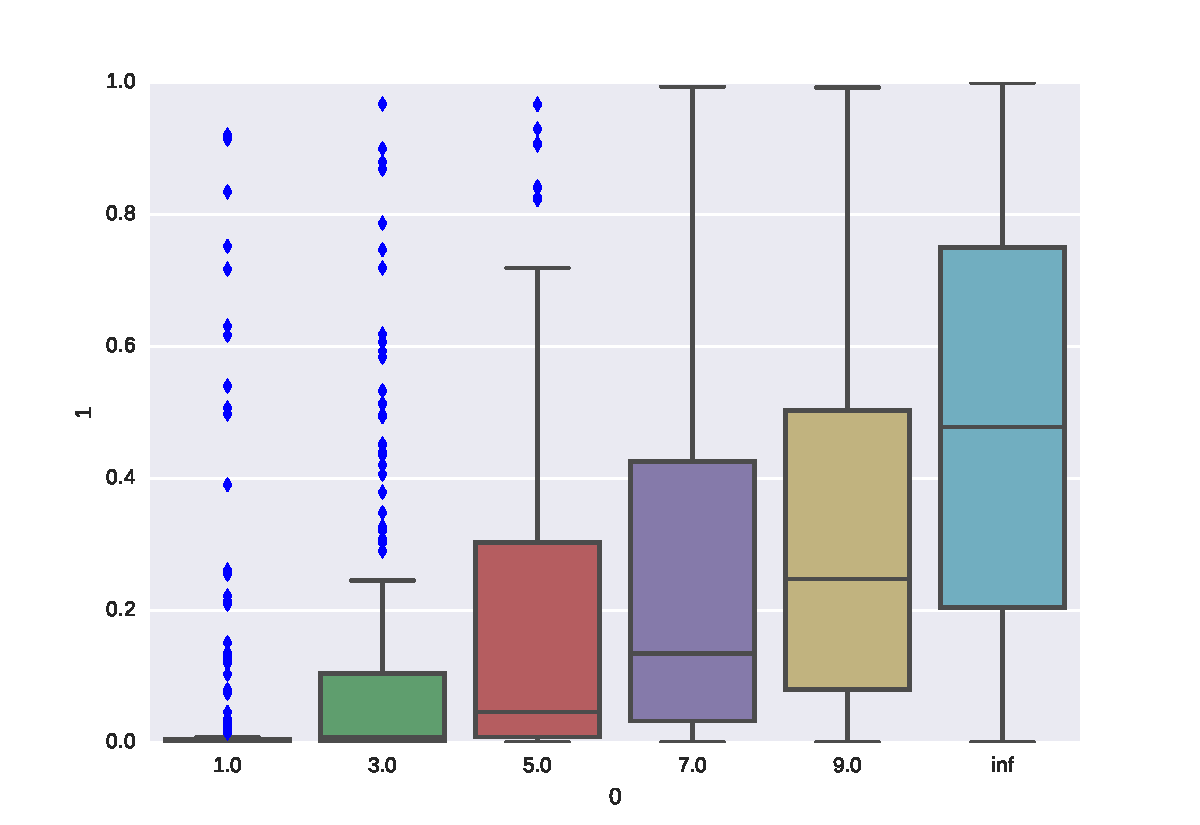
\includegraphics[width=0.8\textwidth]{./img/student.pdf}
\caption{Linear Time test. Distribution of p-values as a function of number of degrees of freedom.}
\end{figure}


% \begin{figure}
% \label{fig:studentstq}
% \includegraphics[width=0.8\textwidth]{./img/qstudent.pdf}
% \caption{Quadratic time test. Distribution of p-values as a function of number of degrees of freedom.}
% \end{figure}

\subsection{MCMC diagnostic}
This one sample test can be used for diagnostics of most of the MCMC methods. In the following experiment we will demonstrate how to verify if the samples obtained form two sampling can be assumed to come from the stationary distribution.  

Here we model used in the experiment 5.1. The model is 
\begin{align}
 \theta_1 \sim N(0,10) ; \theta_2 \sim N(0,1)
 X_i \sim \frac {1}{2} N(\theta_1,4) + \frac{1}{2} N(\theta_2,4) 
\end{align}
400 points are drawn from this model. In the following experiment we would like to characterize the average time required for convergence for two different MCMC algorithms. In order to do so we run multiple chains and asses distribution of p-values. Under the null hypothesis p-values should have uniform distribution and, as in the previous experiment, we asses the divergence of the p-values from the uniform by bar plots. Formally for both methods plain MH and SGLD we generate $40 \times 100$ chains. We divide those chains into $40$ groups of $100$ chains and run one-sample tests for for predefined times $t_1,...,t_10$  so that for each of group we get p-values at ten different times. Then we plot those p-values jointly on plots a and b. We don't use thinning.  


\paragraph{Metropolis Hastings with random walk}
We use plain MH MCMC with Gaussian proposal with with standard deviation equal to  $0.2$.   

\subsection{SGLD, plain }
Stochastic gradient  Stochastic Gradient Langevin Dynamics  with schrinking step size $\epsilon_t$ is a MCMC procedure desigend for large datasets. 
400 points are drawn from the this model with $\theta_1 = 0$ and $\theta_2= 1$. In such a setting there are two modes in the posteriori disitbiution, one at the the point $0,1$ and the other at the point $1,-1$. We run the SGLD alogrithm with a batch size of 1 and 10000 iterations through the whole dataset. The stepsizes are $\epsilon_t = a(b+t)^{.55}$ where $ a = 0.01584$ and $b=2.31$ such that $\epsilon_t$ deacreses from $0.01$ to $.
0001$. 


\begin{figure}
\begin{subfigure}{.5\textwidth}
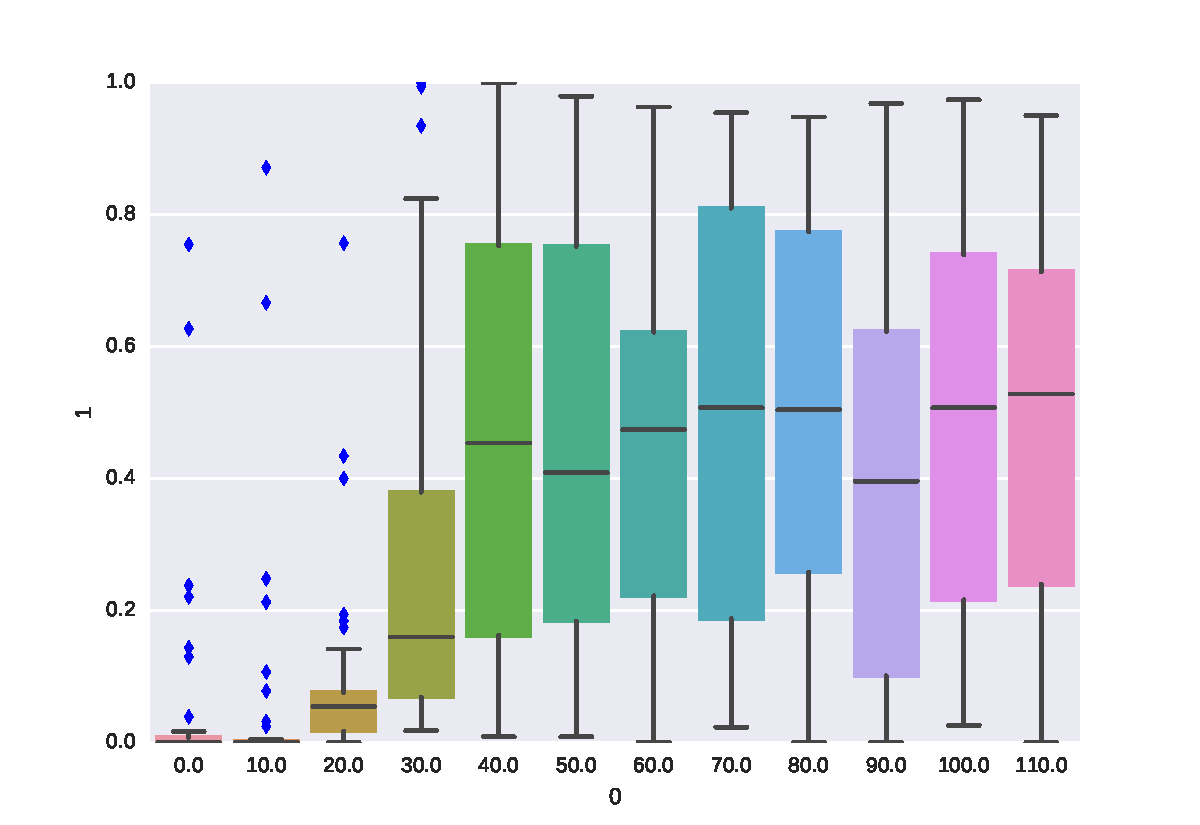
\includegraphics[width=\textwidth]{./img/mcmc_mixing.pdf}
\end{subfigure}%
\begin{subfigure}{.5\textwidth}
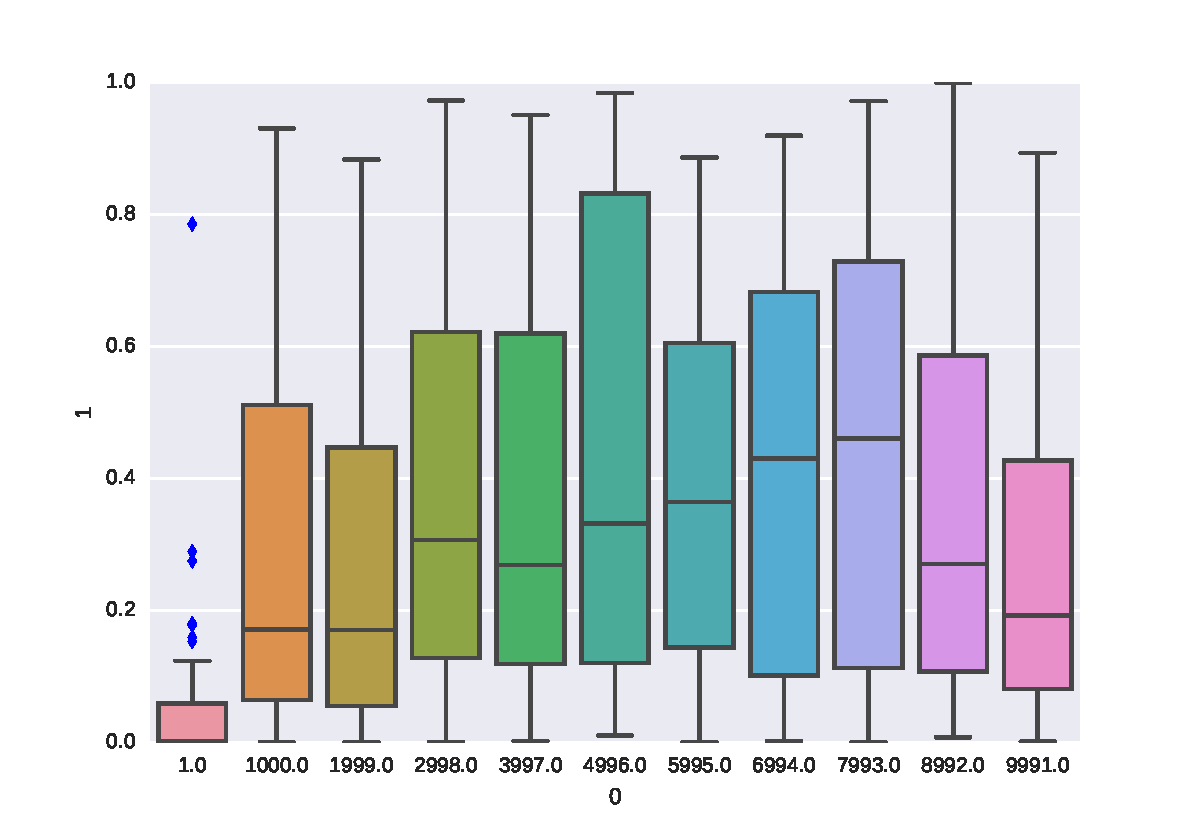
\includegraphics[width=\textwidth]{./img/sgld_mixing.pdf}
\end{subfigure}%
\end{figure}


\begin{figure}
\begin{subfigure}{.5\textwidth}
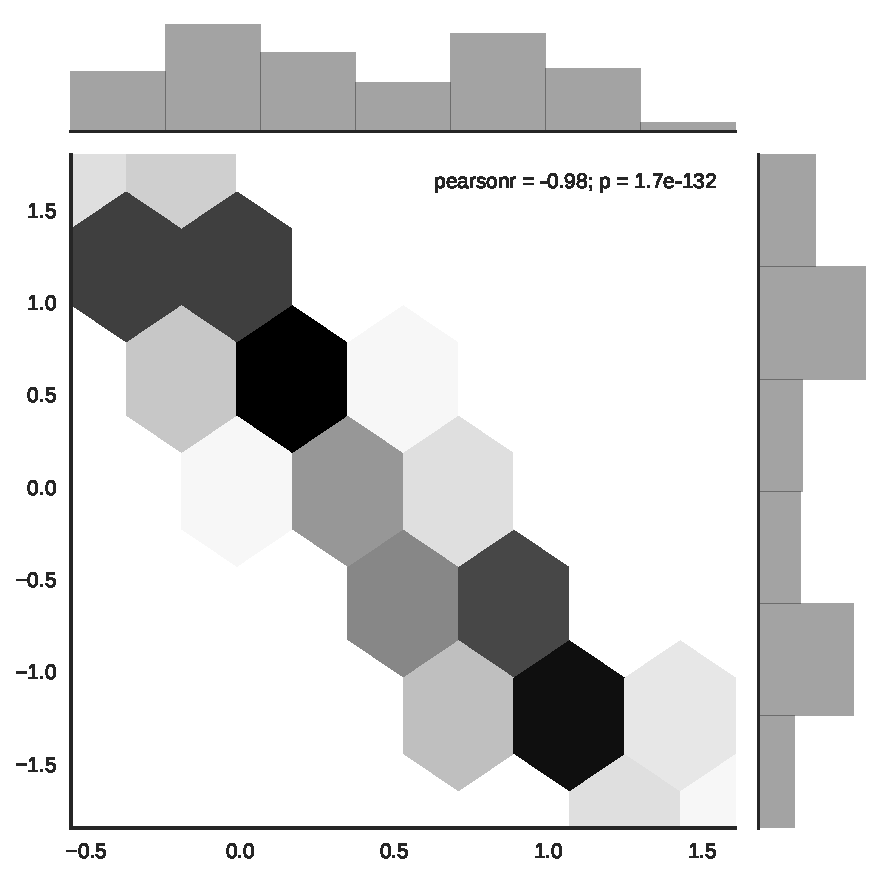
\includegraphics[width=\textwidth]{./img/mcmc_sample.pdf}
\end{subfigure}%
\begin{subfigure}{.5\textwidth}
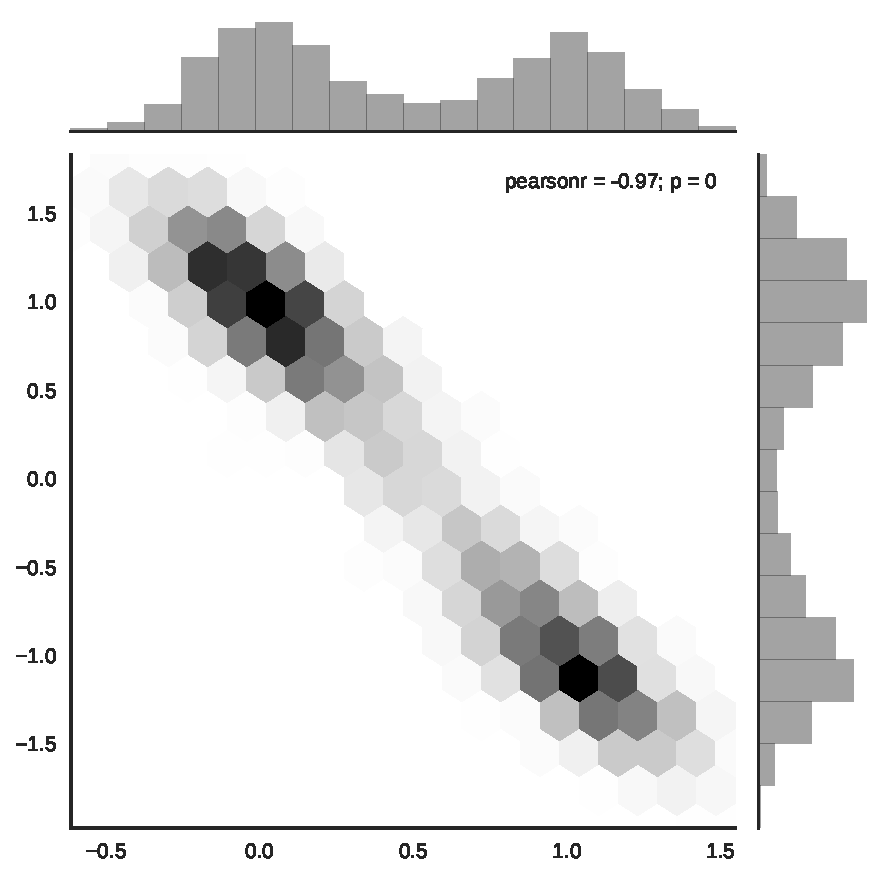
\includegraphics[width=\textwidth]{./img/sgld_sample.pdf}
\end{subfigure}%
\end{figure}




\section{Math}

\begin{statement}
 If $X$ is distributed according to $p$ then the function  $\mu_p(y)$ is identically equal to zero  
\end{statement}
\begin{proof}
 For a fixed $y$ this is consequence of Stein method with as described in those guys NIPS paper. Or one can do integration by parts.   
\end{proof}

\begin{statement}
 If $X$ is not distributed according to $p$, but has a density, then $\mu_p(y)$ is different form zero almost everywhere. 
\end{statement}
\begin{proof}
THIS IS A SKETCH-- which means it's technically not a proof, but you may convince yourself it's true (if it is, but code seems to approve).
 Suppose $X$ is distributed according to density $p'$, then

\begin{align}
\mu_p(y) =& \int_{R^d} ( \nabla \log p(x) g(x,y) -  \nabla g(x,y)) p'(x) dx \\
          & \int_{R^d} g(x,y) \frac{ p'(x)}{p(x)} \nabla p(x) - \nabla g(x,y) p'(x)  
\end{align}
Integration by parts and shows that for all partial derivatives 
\begin{align}
0 = \int_{R} \frac{ \partial g(x,y)p'(x)} { \partial x_i } dx_i
\end{align}
\begin{align} 
 \int_{R} \frac{ \partial g(x,y) } { \partial x_i } p'(x) d x_i =
 -\int_{R} \frac{ \partial p(x) } { \partial x_i } g(x,y) d x_i 
\end{align}
So
\begin{align}
\mu_p(y) =& \int_{R^d} g(x,y) \frac{ p'(x)}{p(x)} \nabla p(x) -  g(x,y) \nabla p'(x)  \\
	 =& \int_{R^d} g(x,y) \left( \frac{ p'(x)}{p(x) } \nabla p(x) -  \nabla p'(x) \right)
\end{align}
 We would like to say that $t(x) = \frac{ p'(x)}{p(x) } \nabla p(x) -  \nabla p'(x)$  is kind of bounded and invoke the argument that $\mu_p$ is analytic, but first we need to prove that $t(x)$ is non-zero. 
 It is sufficient to see that $t(x) =0$ implies that $\nabla [ \log( p(x)) - \log( p'(x)) ]=0$, which implies that $p(x) = p'(x)e^C$. Since both $p$ and $p'$ are probability measures,  $C$ must be equal to 0.
 
 $\mu_p$ lives in the $RKHS$ associated with kernel $g$. Indeed if the integral exists 
 \[
  \int f(x) t(x) 
 \]
 then there exist an element $\mu_t$, such that $<\mu_t, f>$ is equal to above integral and in addition to that 
 \[
  \mu_t(t) = < \mu_t, k(t,\cdot)> = \int k(t,x) t(x) = \mu_p(t). 
 \]
The sufficient condition for $\int f(x) t(x)$ to exist is that 
\[
 \int <f, k(x,)> t(x) = < f, \int k(x,) t(x) > 
\]
$\int k(x,) t(x) $ exists and this one is easily verifiable for popular kernel (e.g. exists for exponential families and Gaussian kernel). By the lemma form our previous paper we see that $\mu_p(t)$ is  analytic. 
\end{proof}

\paragraph{Temporal dependence -- not an issue}
There are several ways to deal with temporal dependence, all of which, to our knowledge, work only asymptotically. Options include estimating auto-covariances, performing bootstrap or thinning. The last one, usually avoided in time-series analysis due to it's wasteful approach to data, is quite feasible in this application. It is also equally or less computationally complex then other options (potentially less noisy then estimating the auto covariance).      

It's obvious, but needs to show formally, that distribution of the test statistic under the null hypothesis, as $n$ approaches infinity, is as if we had used IID data. This is proved in appendix.

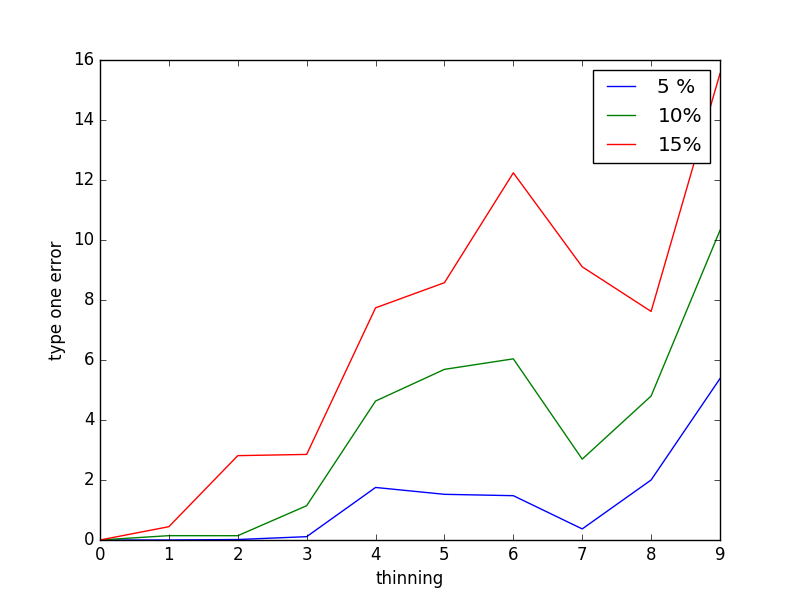
\includegraphics[width=0.8\textwidth]{type1.png}

\section{Sample selection}
So far we have not discussed problem problem of selecting sample from stationary distribution. In this section we propose a procedure that returns a sample for which it can not be rejected that it was generated from null distribution. We will proceed similarly to Heidelberger-Welch procedure, but is simpler way. We will generate blocks of samples and run test on them until we accept of world ends. 

\paragraph{type One-error}
We will use simple Bonferroni correction to deal with type one error. Tests level must be adjusted, so that they sum up to $\alpha$. Any scheme can be used, we use $\frac{1}{x^2}$ since we believe (am I turning  Bayesian?) that chains converge fast on average (faster than precision of the test that we are using).   

\paragraph{Type two}
Type two is somehow more complicated. In general (this is my intuition from finite state Markov chains and AR processes ) chain does not converge to stationary distribution in any number of finite steps, unless it has started for the stationary distribution. As usually in testing, one has no finite sample control over type two error. We can however infer what misspecified log probability would have given similar results on the given sample. This can be done by perturbing log probability in some direction and calculating the statistic on our sample. The magnitude of perturbation will show which models appear to be indistinguishable (now talk about parameters inference and that its even more difficult )    



\appendix

\subsection{boring proofs}

\begin{lemma}
\label{lem:easy}
If a random variable $X$ is distributed according to $p$, then for all function $f \in \mathcal{F}$ expected  value of  $T_p$ is zero, i.e. $\forall_{f \in \mathcal{F}} \ev (T_{q}f)(X) = 0$.
\end{lemma}
\begin{proof}
First we show that the functions $g_i = p \cdot f_i$ vanish at infinity, by which we mean that for all dimensions $j$
\[
 \lim_{x_j \to \infty} g_i(x_1,\cdots,x_d) = 0. 
\]
The density function $p$ vanishes at infinity. The function $f$ is bounded,  which is implied by Cauchy-Schwarz inequality -- $\left|f(x)\right|\le\left\Vert f\right\Vert \sqrt{k(x,x)}$. This implies that the function $g$ vanishes at infinity. To show the expected value $\ev (T_{p})f(X)$ is zero, it is sufficient to show that for all dimensions $i$, the expected value of  $\frac{\partial \log p(X)}{ \partial x_i} f_i(X)+\frac{\partial f_i(X)}{ \partial x_i}$ is zero. 
\begin{align*}
&\ev\left( \frac{\partial \log p(x)}{ \partial x_i} f_i(x)+\frac{\partial f_i(x)}{ \partial x_i} \right) \\
& =\int_{R_d}   \left[ \frac{\partial \log p(x)}{ \partial x_i} f_i(x)+\frac{\partial f_i(x)}{ \partial x_i} \right]q(x)dx\\
 & =\int_{R_d} \left[\frac{1}{p(x)}\frac{\partial q(x)}{ \partial x_i}f(x)  +\frac{\partial f(x)}{ \partial x_i} \right]q(x)dx\\
 & =\int_{R_d} \left[\frac{\partial p(x)}{ \partial x_i} f_i(x)+\frac{\partial  f_i(x)}{ \partial x_i}q(x)\right]dx\\
 & \overset{(a)}{=} \int_{R_{d-1}} \left( \lim_{R \to \infty} p(x)f_i(x) \bigg|_{x_i=-R}^{x_i=R} \right) dx_1 \cdots dx_{i-1} \cdots dx_{i+1}  \cdots d{x_d} \\
 & = \int_{R_{d-1}} 0 dx_1 \cdots dx_{i-1} \cdots dx_{i+1} \cdots d{x_d} \\
 & =0.
\end{align*}
For the equation (a) we have used integration by parts and fact that $g_i$ vanishes at infinity.
\end{proof}


\subsection{Linear time}

For some fixed location $y$ and a random variable $X$, define a random variable $s(X,y)$
\begin{align}
 s(X,y) = \nabla \log p(X) g(X,y) -  \nabla g(X,y).
\end{align}
For some number of random locations $Y_1,Y_J$ and a random variable $X$ define a random vector $Z_i$
\begin{equation}
 Z_i = ( s(X_i,Y_1) , \cdots, s(X_i,Y_J)  )\in \mathbf R^J.
\end{equation}

Let $W_n$ be a mean of $Z_i$'s
$W_n = \frac 1  n \sum_{i=1}^n Z_i, $
and $\Sigma_n$ its  covariance matrix
$\Sigma_n = \frac 1  n Z Z^{T}$.
The test statistic is
\begin{equation}
 S_n = n W_n \Sigma_n^{-1} W_n.
\end{equation}
The computation of $S_n$ requires inversion of a $J\times J$ matrix $\Sigma_n$, but this is fast and numerically stable: $J$ will typically be small, and is less than 10 in our experiments. The next proposition demonstrates the use of $S_n$ as a one-sample test.
\begin{proposition}[Asymptotic behavior of $S_n$]
\label{prop:Hotelling}
 If  $\ev s(X,y)=0$ for all $y$, then the statistic $S_n$ is a.s. asymptotically distributed as a $\chi^2$-random variable with $Jd$ degrees of freedom, where $d$ is $X$ dimensionality (as $n \to \infty$ with $d$ fixed). If  $\ev s(X,y) \neq 0$ for almost all $y$ then a.s. for any fixed $r$, $\mathbb P(S_n > r) \to 1$  as $n \to \infty$ .
\end{proposition}


\begin{test}[One sample test]
\label{test}
Calculate $S_n$. Choose a threshold $r_\alpha$ corresponding to the $1-\alpha$ quantile of a  $\chi^2$ distribution with $J$ degrees of freedom, and reject the null hypothesis whenever $S_n$ is larger than $r_\alpha$. 
\end{test}



\bibliographystyle{plain}
\bibliography{bib}










\end{document}


